% Intrinsic Efficiency
\documentclass[draftcls,onecolumn]{IEEEtran}

%% INCLUDING THE PREAMBLE
%%%%%%%%%%%%%%%%%%%%%%%%%%%%%%%%%%%%%%%%%%%%%%%%%%%%%%%%%%%%%%%%%%%%%%%%%%%
%                                                                         %
%                                 PREAMBLE                                %
%                                                                         %
%%%%%%%%%%%%%%%%%%%%%%%%%%%%%%%%%%%%%%%%%%%%%%%%%%%%%%%%%%%%%%%%%%%%%%%%%%%

%% PACKAGES
\usepackage[]{lineno}
%\linenumbers
\usepackage[usenames,dvipsnames]{xcolor}
\usepackage{microtype}
\usepackage[obeyDraft]{todonotes}
\usepackage{fancyvrb}
\VerbatimFootnotes
\usepackage{algorithmic}

%% GRAPHICS RELATED
\usepackage{graphicx}
\usepackage[outdir=./tmp/]{epstopdf}
\graphicspath{{../images/}{./}{./tmp/}}
\DeclareGraphicsExtensions{.eps, .pdf, .jpeg, .png,}

%% CPATION SETUP
\usepackage{float}
\usepackage{caption}
\usepackage{subcaption}
\captionsetup{belowskip=12pt,aboveskip=4pt}


%% BIBLIOGRAPHY
\bibliographystyle{ieeetr}

%% UNITS
\usepackage{siunitx}

%% EQUATIONS
\usepackage{amsmath}
%\numberwithin{equation}{section}

%% HYPERLINKS
\usepackage[debug]{hyperref}

%%%%%%%%%%%%%%%%%%%%%%%%%%%%%%%%%%%%%%%%%%%%%%%%%%%%%%%%%%%%%%%%%%%%%%%%%%%
%                                                                         %
%                             Listing Setup                               %
%                                                                         %
%%%%%%%%%%%%%%%%%%%%%%%%%%%%%%%%%%%%%%%%%%%%%%%%%%%%%%%%%%%%%%%%%%%%%%%%%%%
\usepackage{listings}
\lstset{ %
    language=C++,
    basicstyle=\footnotesize\ttfamily,
    numbers=left,
    numberstyle=\tiny\color{gray},
    stepnumber=2,
    numbersep=5pt,
    backgroundcolor=\color{white},
    showspaces=false,
    showstringspaces=false,
    showtabs=false,
    frame=single,
    rulecolor=\color{black},
    tabsize=2,
    breaklines=true,
    breakatwhitespace=false,
    title=\lstname,
    keywordstyle=\color{blue},
    commentstyle=\color{OliveGreen},
    stringstyle=\color{orange}
}
\DeclareCaptionFont{white}{\color{white}}
\DeclareCaptionFormat{listing}{\colorbox[cmyk]{0.43, 0.35, 0.35, 0.01}{\parbox{\dimexpr\textwidth-2\fboxsep\relax}{#1#2#3}}}
\captionsetup[lstlisting]{format=listing,labelfont=white,textfont=white,singlelinecheck=false,margin=0pt,font={bf,footnotesize}}
%\lstnewenvironment{code}[1][]%
%{ \noindent\minipage{\linewidth}
%	\lstset{#1}
%}
%{\endminipage}
%% USER COMMANDS
\usepackage{isotope}
\newcommand{\iso}{\isotope}
\newcommand{\figurewidth}{\textwidth}
\newcommand{\micron}{$\mu$m}


% index generation
\usepackage{makeidx}
\usepackage{exercise}
\makeindex
 
% 'list of notations' generation
\usepackage[refpage]{nomencl}  % refer to the page where notation appears
\newcommand{\definevar}[2]{#1 #2\nomenclature{#1}{#2}}
\renewcommand{\nomname}{List of Notations}
\renewcommand*{\pagedeclaration}[1]{\unskip\dotfill\hyperpage{#1}}
\makenomenclature
 


%% Start of the document
\begin{document}
\title{Intrinsic Efficiency Calculations}
\author{Matthew J. Urffer}
\date{\today}
\maketitle

% Nomenclature
\printnomenclature
\printindex

% Tables of Contents, Figures, Tables
\listoftodos
\tableofcontents
\listoffigures
\listoftables
\lstlistoflistings

The intrisinis efficiency is defined as \eqref{eqn:intEffDef} \cite{knoll_radiation_2009}.
\begin{align}
  \label{eqn:intEffDef}
  \epsilon_{int} = \frac{N_c}{N_i}
\end{align}
where:
\begin{itemize}
  \item[] \definevar{$\epsilon_{int}$}{intrisinic efficinecy},
  \item[] \definevar{$N_c$}{number of counts recorded by the detector}, and
  \item[] \definevar{$N_i$}{quanta of radiation incident upon the detector}.
\end{itemize}
The quanta of radation incident upon the detector can be subdived into two components: the source strength and the solid angle.
The composition of $N_i$ is shown in \eqref{eqn:QuantaIncidentDef}
\begin{align}
  \label{eqn:QuantaIncidentDef}
  N_i = \Omega S_0
\end{align}
where:
\begin{itemize}
  \item[] \definevar{$S$}{source strength}, and 
  \item[] \definevar{$\Omega$}{solid angle}.
\end{itemize}
In general the source strength according the half-life of the source \eqref{eqn:HalfLife}, where \definevar{$S_0$}{initial source strength}, \definevar{$t_{1/2}$}{half life} and \definevar{$t$}{age of source}.
\begin{align}
  \label{eqn:HalfLife}
  S = S_0 e^{-\frac{\ln{2}}{t_{1/2}} t}
\end{align}

The solid angle factor is computed using MCNPX. 
A F1 tally is used over the detector surface with two cosine bins, $-1<\cos\theta<0$ and $0<\cos\theta<1$.
As macrobodies are used for the surfaces of the detector, $-1<\cos\theta<0$ represents the particles that cross into the surface and $0<\cos\theta<1$ the particles that leave the surface.
The MCNPX simulation was benched marked against GS20 and against polymer films.
Tables are provided for common geometries, other geometries can be found by interpolatation.

It is often deseriable to express the intrisinic efficiency for a given channel number or Mathmatical Lower Level Discriminator (MLLD)\footnote{The MLLD behaves essentially as a physical lower level discriminator in that all counts below this value are discarded}.
The intrinisinic efficiency can then be expressed as a function of this MLLD \eqref{eqn:MLLDDef}.
The number of counts recorded by the detector can be expressed as the integral of the \definevar{$p(x)$}{spectra function} from some lower bound (the MLLD) to an upper bound, the end of the spectra.
This \eqref{eqn:MLLDDef} is normalized by the incident flux as calculated in \eqref{eqn:QuantaIncident}.
\begin{align}
	\label{eqn:MLLDDef}
	\epsilon &= \frac{\int_{MLLD}^\infty p(x)dx}{N_i}
\end{align}

\subsection{Neutron Intrinsic Efficiency}
The number of counts upon a detector is measured using the neutron irridiator facility.
The quanta of radiation incident upon the detector is found from MCNPX calculations.
This consits of two parts: 1) determining the number of neutrons crossing the detector surface in the lead and cadmium wells and, 2) determining the sourse strength.

The \iso[252]{Cf} source was \SI{0.59}{\ug} on July 2, 2009.
Given that the half-life of \iso[252]{Cf} is 2.65 years and \iso[252]{Cf} has a spontanous neutron emission rate of \SI{2.3E6}{neutron\per\second} the source strength at any given time can be calucalted as \eqref{eqn:Cf252SourceStrength}.
\begin{align}
  \label{eqn:Cf252SourceStrength}
  S &= S_0 e^{-\frac{\ln{2}}{t_{1/2}} t} \\ \notag 
    &= \SI{0.59}{\ug} \iso[252]{Cf} \frac{\SI{2.3E6}{neutron\per\second}}{\si{\ug} \iso[252]{Cf}} e^{-\frac{ \ln{2}}{\SI{2.54}{year}}t}  \\ \notag
    &= \SI{1.357E6}{neutron\per\second} e^{-\frac{ \ln{2}}{\SI{2.54}{year}}t} 
\end{align}

Table \ref{tab:NeutronSolidAngle} sumerizes the incident flux for a number of differnet detector sizes and heights.

\begin{table}
	\centering
	\caption{Simulated Neutron Solid Angle for Various Film Radii}
	\label{tab:NeutronSolidAngle}
	\begin{tabular}{c | c c}
 		Thickness & \SI{1.27}{\cm} & \SI{2.54}{\cm} \\ \hline
		& & 
	\end{tabular}
\end{table}

It should be noted that there is considerable variation in the neutron flux in the detector wells, as shown in \ref{fig:NeutronFluxProfiles}.
Thus, even though the calculations are accurate to less than a precent, the real error on the intrisinic efficinecy will be much higher due to undertainity in where the detector was placed in the well.
\begin{figure}
	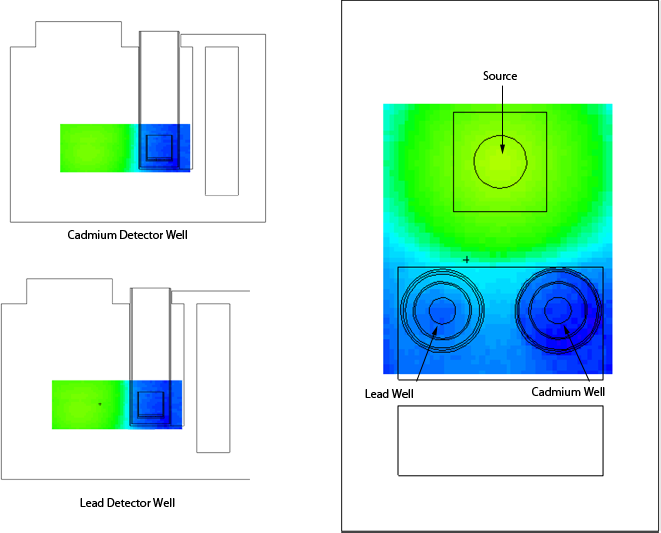
\includegraphics[width=\textwidth]{SpatialNeutronFlux}
  \caption{Neutron Flux Profiles of the Lead and Cadimum Wells}
  \label{fig:NeutronFluxProfiles}
\end{figure}

\subsection{Gamma Intrinsic Efficiency}
The gamma intrinisic efficiency is calculated by a combination of simulation to determine the solid angle that the detector subtends and radioactive decay.
The gamma irridator consits of a \SI{97}{\micro Ci} \iso[60]{Co} on January 1st, 2012.
The incident flux is calcualted according to \eqref{eqn:Co60SourceStrength}, and the solid angle is tabulated in Table \ref{tab:GammaSolidAngle}.
\begin{align}
  \label{eqn:Co60SourceStrength}
  S &= S_0 e^{-\frac{\ln{2}}{t_{1/2}} t} \\ \notag 
    &= \SI{97}{\micro Ci} \iso[60]{Co}\; \frac{\SI{1.3E10}{decay\per\second}}{\si{Ci}} \;\frac{2\text{photon}}{decay}\;e^{-\frac{ \ln{2}}{\SI{5.27}{year}}t}  \\ \notag
    &= \SI{7.178E6}{photon\per\second}\;e^{-\frac{ \ln{2}}{\SI{5.27}{year}}t} 
\end{align}
\begin{table}
	\centering
	\caption{Simulated Gamma Solid Angle for Various Film Radii}
	\label{tab:GammaSolidAngle}
	\begin{tabular}{c | c c}
 		Thickness & \SI{1.27}{\cm} & \SI{2.54}{\cm} \\ \hline
		& & 
	\end{tabular}
\end{table}
The intrisinic efficiency is then found by normalizaling by the amount of  
The gamma irridiator detector well is encased in a 1/2 inch steel pipe which is surrounded by lead, providing a beam like geometry while also introducing lower energy photons. 
The contribution of these lower energy photons is shown if Figure \ref{fig:PhotonFluxAllEnergies}.
\begin{figure}
  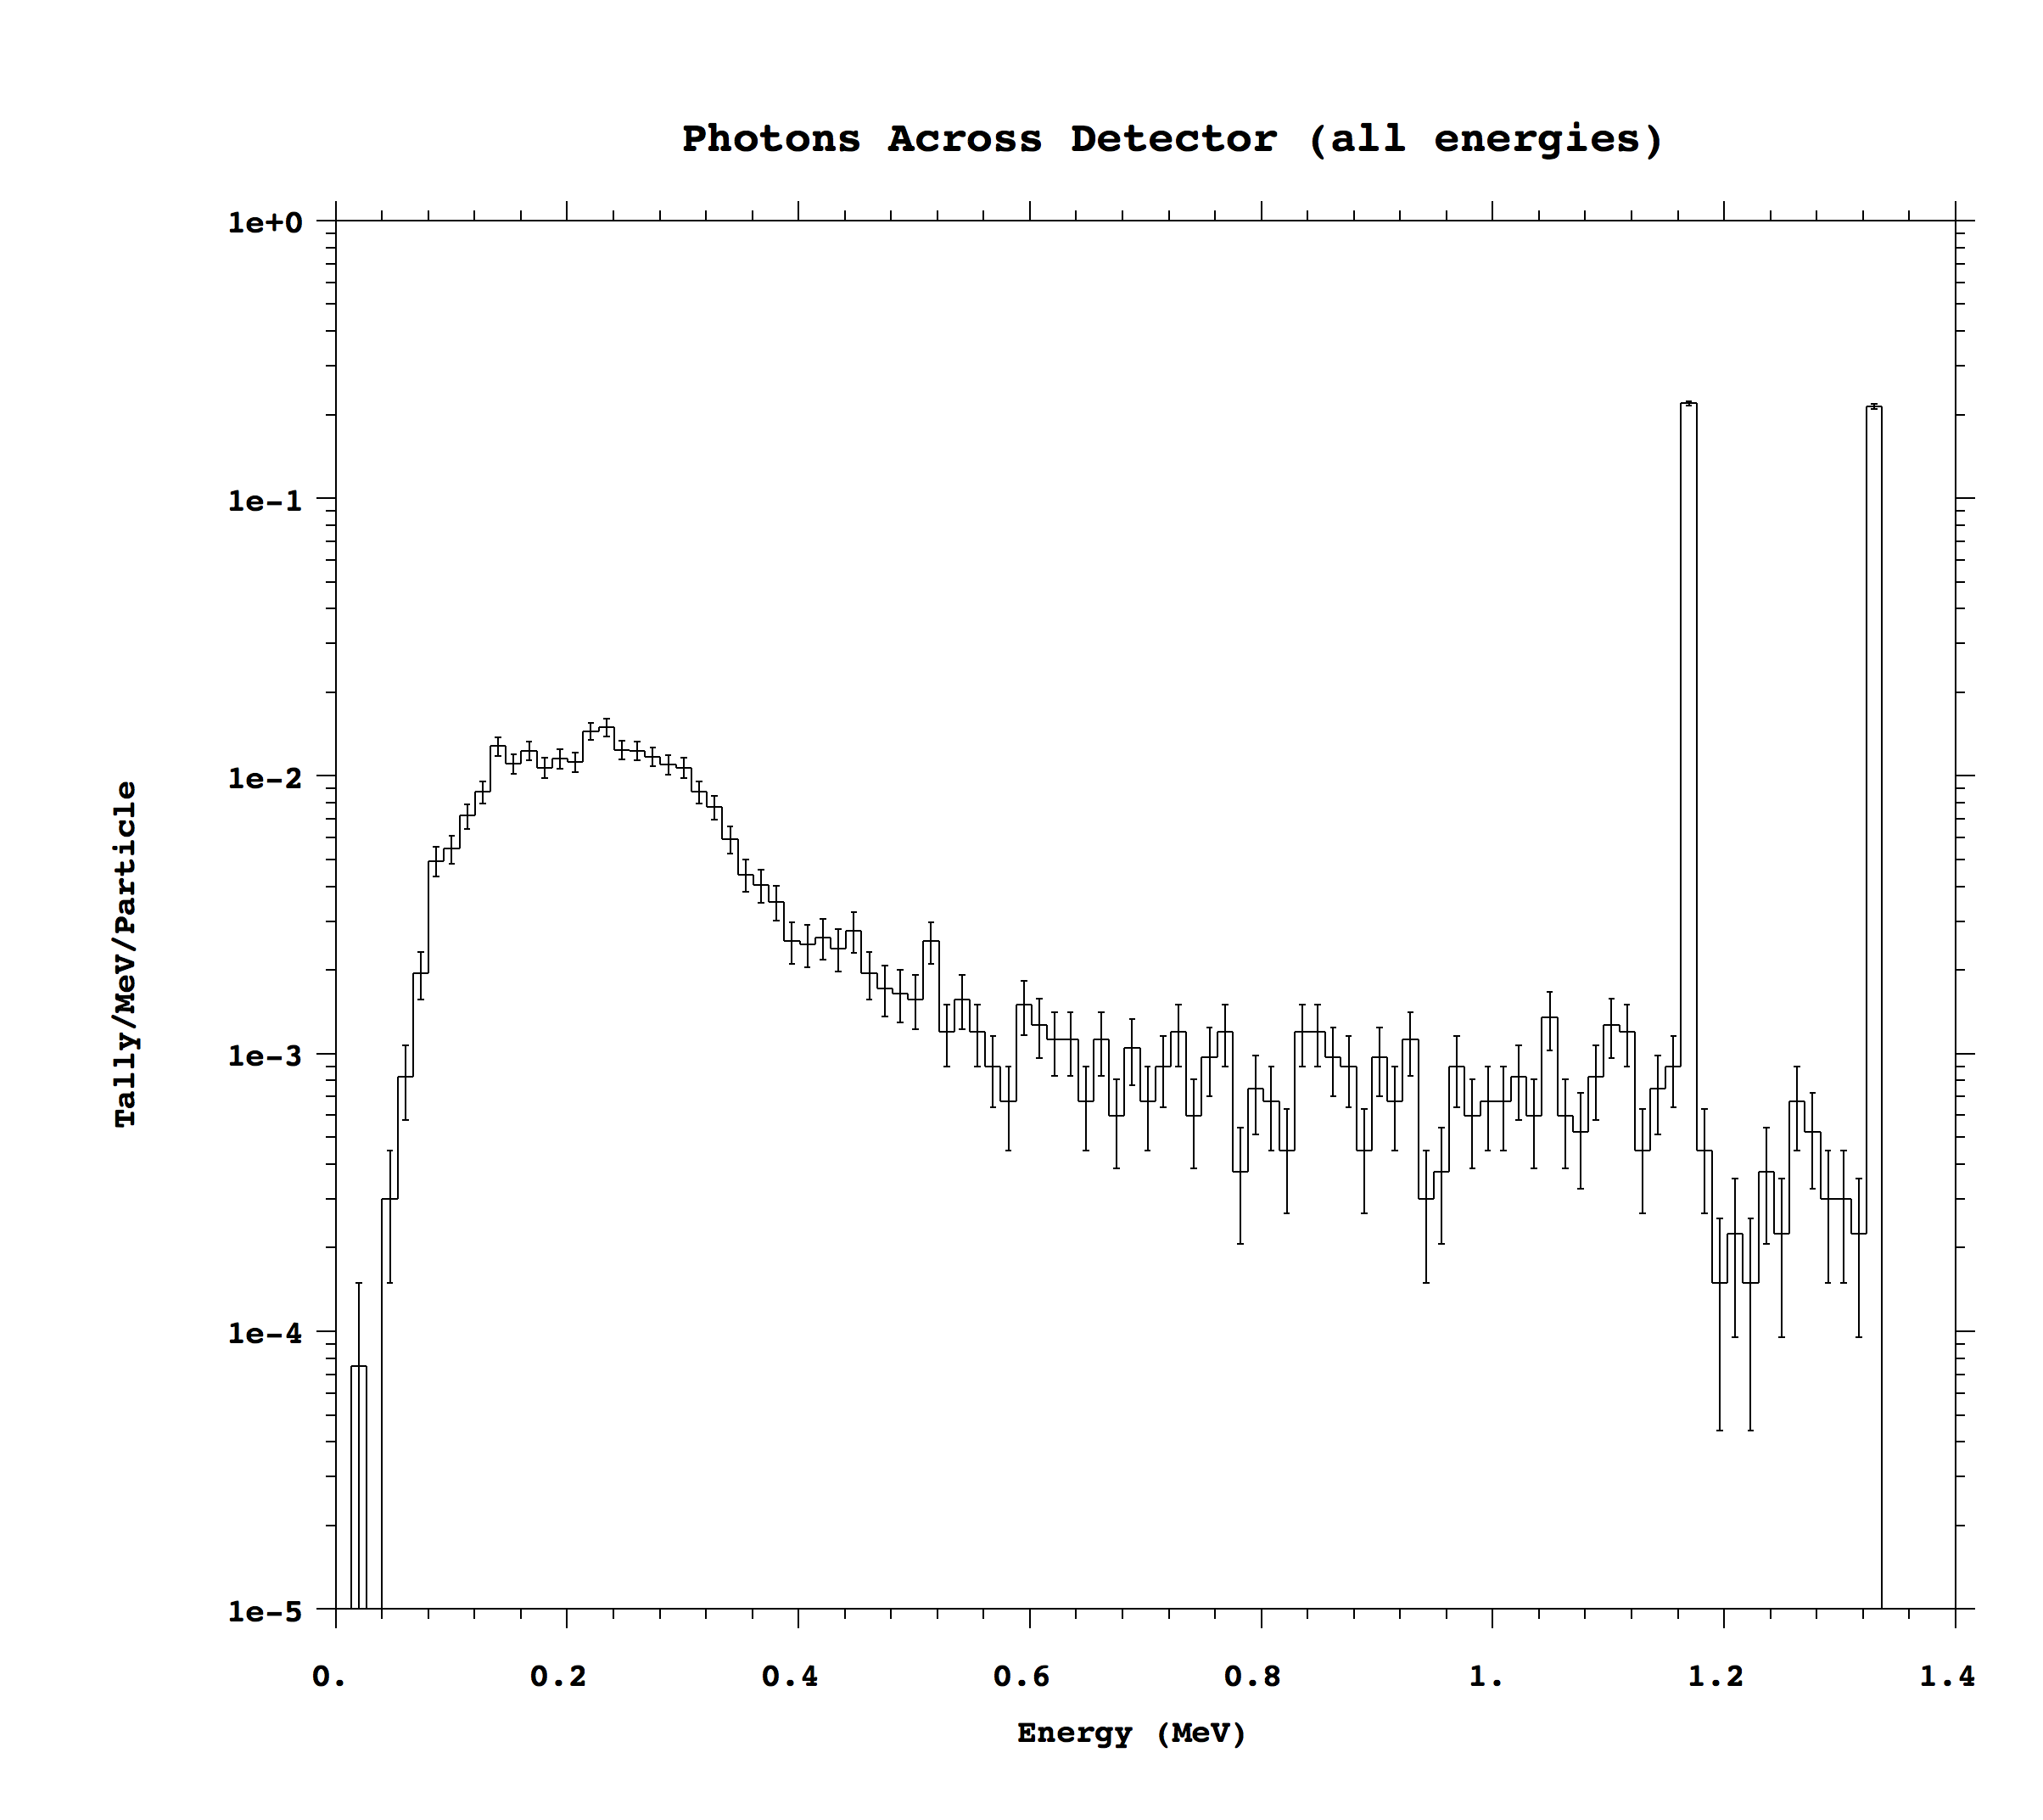
\includegraphics[width=\textwidth]{PhotonEnergyDist}
	\caption{Photon Flux into Detector}
  \label{fig:PhotonFluxAllEnergies}
\end{figure}

\pagebreak
\subsection{Examples}
\begin{Exercise*}[label={LiBorateGlass},title={Li borate glass},name={Example}]
A sample measured on April 4, 2013 \SI{1.327}{\g} sample of $\iso[6]{Li}\text{B}_4\text{O}_7$ glass was fabricated by John Auxier.
This sample was roughly rectanular in shape (\SI{1.3}{\cm} by \SI{2.2}{\cm}) with a thickness of \SI{2.7}{\mm}.
The sample was measured April 4, 2013.



The neutron intrisinic efficiency is calcualted according to \eqref{eqn:intEffDef} with the source strength as supplied in \eqref{eqn:Cf252SourceStrength}, with the source aging $t = 3.76 \text{yr}$ to the measurment.
\begin{align}
    S &= \SI{1.357E6}{neutron\per\second} e^{-\frac{ \ln{2}}{\SI{2.54}{year}}\SI{3.76}{year}} \\ \notag
      &= \SI{4.86E5}{neutron\per\second}
\end{align}
Approximating the sample as a cylinder (maintaining the area of the faces) yeilds a radius of \SI{0.95}{\cm}.
\begin{align}
	r &= \sqrt{\frac{\SI{1.3}{\cm} \times \SI{2.2}{\cm}}{\pi}} \\ \notag
	& = \SI{0.95}{\cm}
\end{align}
From Table \ref{tab:NeutronSolidAngle} the closest radius is


The gamma intrisinic efficiency is calcualted according to \eqref{eqn:intEffDef} with the source strength as supplied in \eqref{eqn:Co60SourceStrength} and the solid angle Table \ref{tab:GammaSolidAngle}.
The \iso[60]{Co} source has aged 459 days (1.26 years) since the measurment.
The source strength is then:
\begin{align}
  S &= \SI{7.178E6}{photon\per\second}\;e^{-\frac{ \ln{2}}{\SI{5.27}{year}}\SI{1.26}{year}} \\ \notag
    &= \SI{6.08E6}{photon\per\second}
\end{align}
Once again interplation is used to calculated the solid angle.
\begin{align}
A = B
\end{align}
\end{Exercise*}

% Bibliography
\bibliography{../Zotero}

\Appendix
The generated MCNPX tables was based upon a script input deck for gamma and neutrons in \verb+MCNP/IncidentFlux+.
An analysis script was written in python in order to extract the necessary lines from the output decks.
\end{document}

